\graphicspath{{RL/fig}}
\chapter{Reinforcement Learning}
\label{chap:RL}

In previous chapters we discussed methods which required knowledge about the model of the environment. This knowledge was embedded in the probability transition matrix P. Often times it is not possible to know the model of the environment beforehand. This is where reinforcement learning is useful because it does not require a model of the environment.

In reinforcement learning, the way an agent learns the best actions to take, is by experiencing sequences of states and actions, defined as an episode. When the agent reaches the final state, we say the episode has terminated. In this chapter we discuss two methods of reinforcement learning (Monte Carlo and temporal difference methods), both of which can be implemented via prediction or control methods. We will not cover the Monte Carlo control method, but it can be found in Sutton and Barto \cite{sutton_barto}. We begin in the next section with the prediction methods.
\section{Model-free prediction}
\subsection{Monte Carlo prediction}
According to Sutton and Barto the term Monte Carlo is generally used for
any estimation technique where a large portion of its operation is random \cite{sutton_barto}.
Sutton and Barto specifically describes Monte Carlo methods as solving reinforcement learning problems by averaging sample returns \cite{sutton_barto}.
Monte-Carlo methods require only experience, which it obtains by sampling sequences of states, actions and rewards. By sampling enough times, by the law of large numbers, eventually an accurate state-value function will be obtained  \cite{sutton_barto}.

Monte-Carlo policy evaluation works as follows. We define a total return S in state s as S(s) and a integer counter N(s) which represents the amount of times s is seen. We then initialize both S(s) and N(s) initialized to zero. 
Then at time step t and state s we increment the counter N(s) = N(s)+1. This can be done in two ways, one being only incrementing N(s) the \textit{first} time state s is seen, the other being incrementing N(s) \textit{every} time states s is seen \cite{sutton_barto}.

In this chapter we use the method of incrementing the counter every instance that state s is seen.
Then we increment the total reward S(s) =  S(s) + $G_t$ every time the agent reaches state s.
Finally we calculate the state value estimate function as $V(s)=\frac{S(s)}{N(s)}$.
Then $V(s) \to V_\pi(s)$ as N(s) $\to \infty$,  $\forall$ s $\in$ S. In other words when we have seen all states infinitely many times, we will have obtained exactly $V_\pi(s)$. Although theoretically we need to visit each state infinitely many times, practically there is a finite time-step where $V(s)$ converges to $V_\pi(s)$.
In order to describe incremental Monte-Carlo updates, David Silver introduces the concept of an incremental mean $u_k$ \cite{David_Silver}. The derivation for $u_k$ from a standard mean is as follows:
\begin{align}
	u_k &= \frac{1}{k}\sum_{j=1}^{k}x_j\\
	&= \frac{1}{k}(x_k + \sum_{j=1}^{k-1}x_j) \nonumber\\
	&= \frac{1}{k}(x_k +(k-1)u_{k-1})\nonumber\\
	&= u_{k-1} + \frac{1}{k}(x_k - u_{k-1}).
	\label{eq:u_k}
\end{align}
Since V(s) is a mean, we break it up similarly to Equation \ref{eq:u_k}, with $u_{k-1}=V(s)$, $N(s)=t=k$ and return $G_t =x_k$. Substituting these variables into equation \ref{eq:u_k} yields that at every time-step t:

\begin{align}
	N(S_t) &\gets N(S_t) + 1 \\
	V(S_t) &\gets V(S_t) + \frac{1}{N(S_t)}(G_t - V(S_t)).
\end{align}
Sutton and Barto in \cite{sutton_barto} sets $\frac{1}{N(S_t)}=\alpha$, where $0<\alpha<1$ resulting in
\begin{equation}
	V(S_t) \gets V(S_t) + \alpha(G_t - V(S_t)).
	\label{eq:monte_carlo}
\end{equation}
Equation \ref{eq:monte_carlo} gives us a way to find the optimal state-value function $V_\pi(S_t)$ by iteratively updating $V(S_t)$. Sutton and Barto names Equation \ref{eq:monte_carlo}, $constant-\alpha$ Monte Carlo.

\subsection{Temporal Difference (TD) Learning}
Temporal difference (TD) learning uses a combination of Monte Carlo and dynamic programming (DP) ideas. TD is one of the unique aspects of reinforcement learning, unlike Monte Carlo and DP which have more general applications besides reinforcement learning \cite{sutton_barto}. Like Monte Carlo TD learns without requiring a model of the environment. Because TD is a reinforcement method, it can be split into prediction and control methods as was stated in the introduction of this chapter. Here in this section we only describe the prediction method, while the next section will discuss two TD control methods, namely SARSA and Q-learning. The aim of TD learning is to learn a value function $v_\pi$ from experience by following policy $\pi$. 
The simplest form of TD is replacing the return $G_t$ in Equation \ref{eq:monte_carlo} from the previous section as follows:
\begin{equation}
	V(S_t) = V(S_t) + \alpha({\color{red}R_{t+1} +  \gamma V(S_{t+1})} - V(S_t)).
	\label{eq:monte_carlo_TD}
\end{equation}
Where $[{\color{red}R_{t+1} +  \gamma V(S_{t+1})}]$ is known as the TD target, the value which $V(S_t)$ tends to as $t \to \infty$ and
$[{\color{red}R_{t+1} +  \gamma V(S_{t+1})} - V(S_t)]$ is known as the TD error. The aim of TD learning is to reduce the TD error to zero and update $V(S_t)$ to the estimated return ${\color{red}R_{t+1} +  \gamma V(S_{t+1})}$.
Suttton and Barto mathematically describes the relationship between MC and TD using what they define as the n-step return $G_{t}^{(n)}$ described by:
\begin{equation}
	G_{t}^{(n)} = R_{t+1} + \gamma R_{t+2} + ... + \gamma^{n-1}R_{t+n} + \gamma^{n}V(S_{t+1}).
	\label{eq:n_step_gt}
\end{equation}
For clarity we show 
$G_{t}^{(n)}$ for a few values of n as follows:\\
\begin{align}
	 {\color{red}(TD)} n &= 1: G_{t}^{(1)} = R_{t+1}+\gamma V(S_{t+1}) \label{eq:td} \\
	n &= 2 : G_{t}^{(2)} = R_{t+1}+ \gamma R_{t+2}+\gamma^2 V(S_{t+2}) \\
	{\color{red}(MC)} n &= \infty : G_{t}^{(\infty)} = R_{t+1}+ \gamma R_{t+2}+...+\gamma^{T-1} R_T. \label{eq:mc_td}
\end{align}
What can be seen is, as n $\to$ $\infty$, the return in TD learning turns into the same form as in Monte Carlo. Hence Monte Carlo can be said to be a special case of TD learning.
Substituting $G_{t}^{(n)}$ into Equation \ref{eq:monte_carlo_TD} yields what Sutton and Barto calls n-step TD as:
\begin{equation}
	V(S_t) \gets V(S_t) + \alpha(G_t^{(n)} - V(S_t)).
	\label{eq:n_step_TD}
\end{equation} 
What we now have is a method to control how many steps we want an agent to look ahead. This is useful because $V(S_t)$ can converge more quickly to $V_\pi(S_t)$ if n is chosen well. Normally one has to test for different values of n to see which value works best for the specific problem at hand.
In the next section we no longer look at estimating the state-value function $V_\pi(S_t)$, but instead work with \textit{state-action} pairs in order to find the optimal state-action function $q_*(s,a)$.

\section{Model-free control}
Model-free control can be implemented in two ways. \textbf{On-policy learning}, which lets the agent learn characteristics of a policy $\pi$ by sampling from $\pi$ and
\textbf{off-policy learning}, learning characteristics of policy $\pi$ by sampling another policy.

\noindent In order to find the optimal state-action function $q_*(s,a)$, we require a method of evaluating a state-action policy. Previously, when using greedy policy improvement over the state-value function V(s) we had in Equation \ref{pi'}:
\[\pi^{'}(s) = \max\limits_{a \in A}(R^{a}_s+\gamma\sum_{s'\in S}P^{a}_{ss'}v_*(s'))\]
Sutton and Barto applies greedy policy improvement over the state action function Q(s,a) as follows:
\begin{equation}
	\pi^{'}(s) = \max\limits_{a \in A}Q(s,a).
	\label{eq:pi'}
\end{equation}
One should notice that to find the optimal policy (by using Equation \ref{eq:pi'} for policy improvement), we no longer need a model of the environment. In other words there is no dependency on the probability matrix $P^{a}_{ss'}$. In the next section we will see that there is a problem if an agent only uses Equation \ref{eq:pi'} for policy improvement. In the same section a solution is then given to the problem.

\subsection{Exploration and exploitation}
In reinforcement learning, exploration refers to an agent taking a random action and exploitation when the agent acts greedily. When an agent exploits it can obtain a larger return and when it explores it gets a more accurate estimate of the action-value function. The agent can not simultaneously explore and exploit which results in what is known as the exploration-exploitation dilemma \cite{e_greedy_Michel_T}.
To ensure that the agent explores occasionally instead of always taking the greedy action with respect to the state-action function Q(s,a), we let the agent act randomly with a probability $\epsilon$. This can mathematically be expressed as:
\begin{align}
	\pi(a|s)=\begin{cases}
		1-\epsilon, & \text{if $a^* = \argmax\limits_{a \in A}Q (s,a)$}\\
		\epsilon, & \text{otherwise take a random action}
	\end{cases}
	\label{eq:pi_epsilon-greedy}
\end{align}
Equation \ref{eq:pi_epsilon-greedy} is known as the $\epsilon$-greedy policy. 
Using the $\epsilon$-greedy policy results in the agent exploring occasionally, which allows for faster convergence if $\epsilon$ is chosen appropriately. Usually, an $\epsilon$ of 0.1 is a good starting value.

\subsection{SARSA: On policy TD control}
\begin{figure}[!htb]
	\centering
	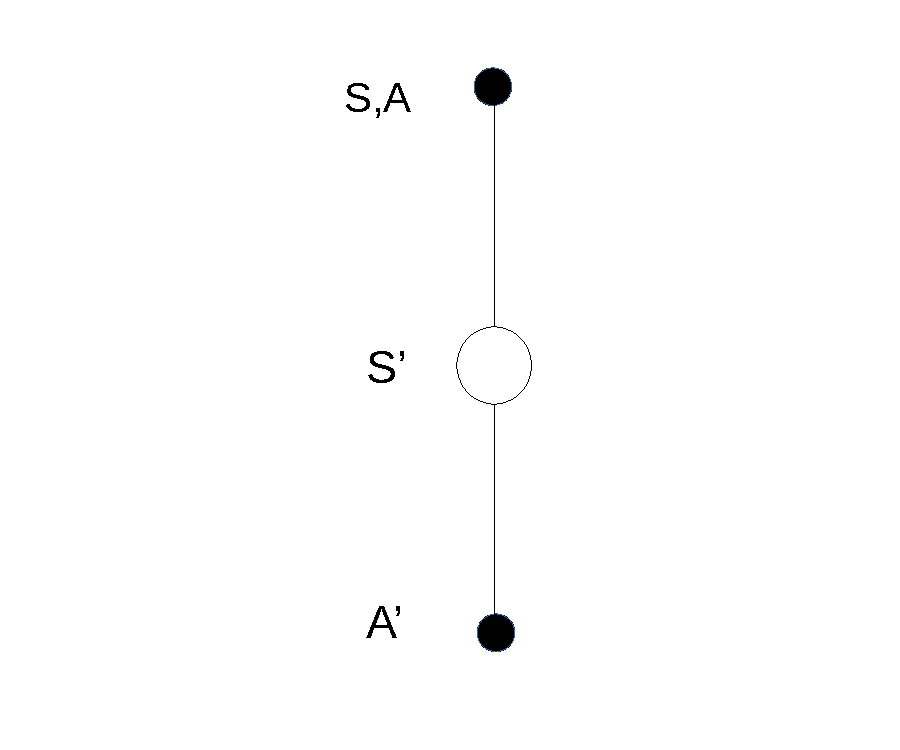
\includegraphics[width=0.5\linewidth]{RL/fig/sarsa_state_diagram.pdf}
	\caption{SARSA backup diagram representation\cite{David_Silver}}
	\label{fig:sarsa_state_diagram}	
\end{figure}

We now look at using TD methods for control. The backup diagram for SARSA is shown in Figure \ref{fig:sarsa_state_diagram}, where we visually see a sequence of a State-Action-Reward-State-Action (SARSA). This is where the name SARSA originates from. By following the same process that we used in the TD prediction section, we can arrive to an equation similar to Equation \ref{eq:monte_carlo_TD}. Instead of updating the state-value function $V(S)$, we update the state-action function $Q(S,A)$. For every state action pair, we can calculate the state-action function Q(S,A) using TD learning as follows:

\begin{equation}
	Q(S,A) = Q(S,A) + \alpha[R+\gamma Q(S',A') - Q(S,A)].
	\label{eq:sarsa_update}
\end{equation}
Where $R+\gamma Q(S',A')$ is the TD target. Similar to Monte Carlo prediction where a n-step state value return $G^n_t$ was defined in Equation \ref{eq:n_step_gt}, Sutton and Barto also defines n-step Q-return as:
\begin{equation}
	q_{t}^{(n)} = R_{t+1} + \gamma R_{t+2} +...+ \gamma^{n-1}R_{t+n}+\gamma^{n}Q(S_{t+n}).
	\label{eq:q_return}
\end{equation}
Although Sutton and Barto do not explicitly mention it, but $q_{t}^{(n)}$ is assumed to be zero for all $n < 1$.
The goal of n-step SARSA is to update Q(s,a) towards the n-step Q-return $q_t^{(n)}$,
\begin{equation}
	Q(S_t,A_t) = Q(S_t,A_t) + \alpha[q_{t}^{(n)} - Q(S_t,A_t)].
	\label{eq:sarsa_n_step}
\end{equation}
Sutton and Barto states that SARSA always converges towards an optimal action-value function, as long as all state–action
pairs are visited enough times \cite{sutton_barto}. One can also deduce this fact from the law of large numbers, as was stated in the Monte Carlo prediction section.

Algorithm \ref{alg:SARSA} below, adapted from Sutton and Barto, shows the pseudo-code which can be used to implement SARSA. Lines 4 and 7 in algorithm \ref{alg:SARSA} is policy improvement. Line 8 is the SARSA update line corresponding to Equation \ref{eq:sarsa_n_step}, with n=1. Later in chapter \ref{chap:Experiments_and_Results} we will apply this algorithm, where will adjust the hyper parameters to see how they affect the agents learning process.

\begin{algorithm}
	\SetKwInOut{Input}{Input}
	\SetKwInOut{Output}{Output}
	\caption{SARSA algorithm to find optimal state action function $Q_*(S,A)$}	
	\underline{function SARSA $(\alpha,\gamma,\epsilon)$}\;
	\Input{Three nonnegative integers, learning rate $\alpha$, discount $\gamma$ and exploration probability $\epsilon$}
	\Output{$Q(S,A)$}

	\begin{algorithmic}[1]
		\State Initialize Q(s,a), $\forall$s$\in$S, a$\in$A(s) arbitrarily and Q(terminal state, \{all actions\}) = 0
		\State for each episode:
			\State \hskip2.0em Initialize S
			\State \hskip2.0em Choose A from S using $\epsilon$-greedy policy derived from Q  
			\State \hskip2.0em for each step in episode:
				\State \hskip6.0em Take action A, observe R,S'
				\State \hskip6.0em  Choose A' from S' using $\epsilon$-greedy policy derived from Q
				\State \hskip6.0em Q(S,A) $\gets$ Q(S,A) + $\alpha$[R + $\gamma$(Q,S',A') - Q(S,A)]
				\State \hskip6.0em S $\gets$ S'; A $\gets$ A';
			\State \hskip2.0em Until S is terminal
	\end{algorithmic}
	\label{alg:SARSA}
\end{algorithm}
\newpage
\subsection{Q-learning: Off policy TD control}
\begin{figure}[!htb]
	\centering
	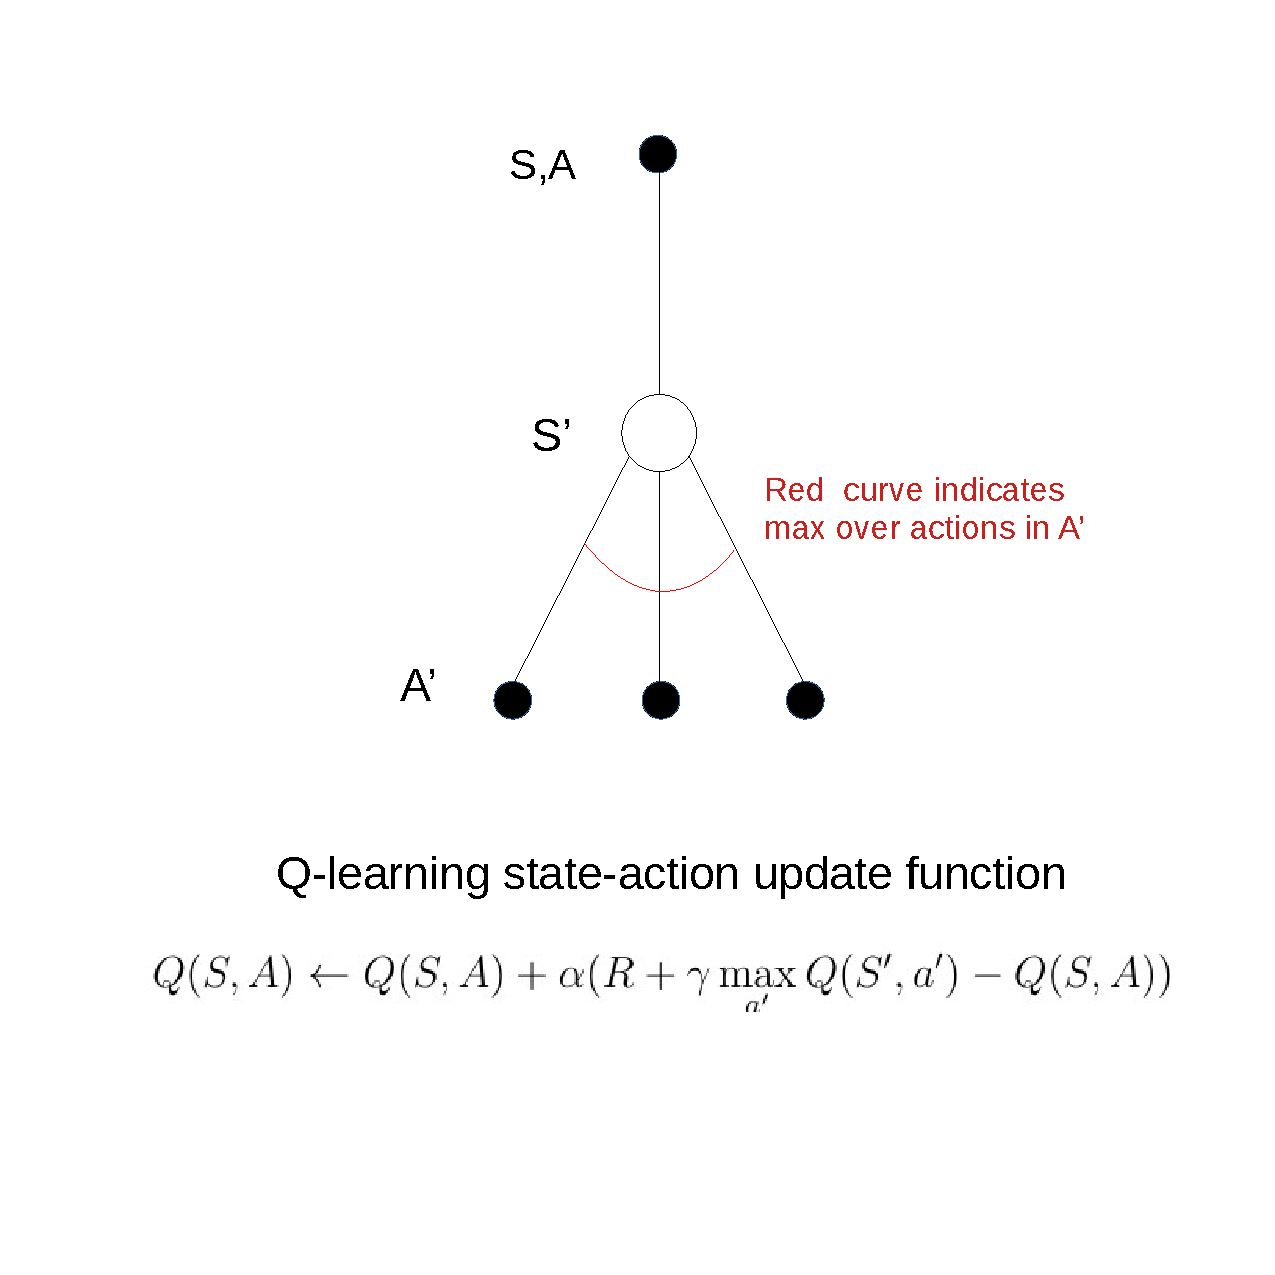
\includegraphics[width=0.5\linewidth]{RL/fig/q_learning_state_diagram.pdf}
	\caption{Q-learning backup diagram where the red line indicates a max across the actions that can be taken from state S'\cite{David_Silver}}
	\label{fig:q_learning_state_action_diagram}
\end{figure}
\begin{equation}
	Q(S,A) \leftarrow Q(S,A) + \alpha(R + \gamma\max\limits_{a'}Q(S',a') - Q(S,A)).
	\label{eq:q_learning_update_function}
\end{equation}
We describe now Q-learning which falls under off policy learning. What we have been dealing with up to this chapter, was on-policy learning. Q-learning is an off-policy method, because it not only updates Q(S,A), but it also updates the TD target $[R + \gamma\max\limits_{a'}Q(S',a')]$. By comparing Figure \ref{fig:q_learning_state_action_diagram} and Figure \ref{fig:sarsa_state_diagram}, we can see that the only difference between Q-learning and SARSA is that Q-learning takes the action a', which results in the maximum state-action function $Q(S',a')$. We will also apply the Q-learning algorithm in Chapter \ref{chap:Experiments_and_Results}. In this chapter we have covered various methods of reinforcement learning, of which we will only be applying TD control methods, namely SARSA and Q-learning. In the next chapter we will also discuss what effects each hyper parameter has on th agents learning process.\\
\begin{algorithm}[H]
	\SetKwInOut{Input}{Input}
	\SetKwInOut{Output}{Output}
	\caption{Q-learning algorithm to find optimal state action function $Q_*(S,A)$}	
	\underline{function Q-learning $(\alpha,\gamma,\epsilon)$}\;
	\Input{Three nonnegative integers, learning rate $\alpha$, discount $\gamma$ and exploration probability $\epsilon$}
	\Output{$Q(S,A)$}
	
	\begin{algorithmic}[1]
		\State Initialize Q(s,a), $\forall$s$\in$S, a$\in$A(s) arbitrarily and Q(terminal state, \{all actions\}) = 0
		\State for each episode:
		\State \hskip2.0em Initialize S
		\State \hskip2.0em for each state in episode:
		\State \hskip6.0em Choose A from S using policy derived from Q (eg., $\epsilon$-greedy)
		\State \hskip6.0em Take action A, observe R,S'
		\State \hskip6.0em Q(S,A) $\gets$ Q(S,A) + $\alpha$[R + $\gamma$$\max\limits_{a \in A}$(Q,S',a) - Q(S,A)]
		\State \hskip6.0em S $\gets$ S';
		\State \hskip2.0em Until S is terminal
	\end{algorithmic}
	\label{alg:Q_learning}
\end{algorithm}